\chapter{Design and materials}
In this section we will discuss the design of our mechanical, electronic, and software systems and the materials used.

\section{Mechanical design}
The mechanical design consists of three main components: the horizontal movement,  the vertical movement,  and the rotation of the racket. 
The materials utilized are a combination of purchased components such as linear rails, timing belts, bolts, and nuts alongside custom 9mm MDF parts, made by using a laser cutter in FabLab.

The two 1.5-meter-long linear rails are positioned vertically, parallel to each other, along the table's edge to ensure stability and prevent tipping of the system. Three linear rail blocks, which slide along these rails, support the vertical structure of the design. These rail blocks have screw holes, allowing them to be securely connected in a triangular formation using an MDF plate. The vertical structure is mounted on this plate.

A stepper motor is mounted at one corner of the table, fixed to the edge of the rails using MDF. This motor drives a 60-tooth GT2 gear. At the opposite corner, a shoulder bolt with a gear is similarly secured using MDF. A 6mm-wide GT2 timing belt spans between these two gears, and is attached to one of the horizontal rail blocks, allowing horizontal movement by rotating the stepper motor.

The vertical structure is mounted on the horizontal MDF plate, attached to its linear blocks. It includes two 0.5-meter-long aluminium pipe and a vertical MDF plate that stabilizes the pipes. A gear is placed on top of the vertical plate and pipes, held in place with a shoulder bolt. Two vertical rail block are positioned on the pipes, allowing vertical movement. Another stepper motor is attached at the bottom of the horizontal MDF plate, with a gear connected to it. A timing belt spans between the gear on the top and bottom of the structure and is attached to the vertical rail blocks, allowing vertical movement of the block by rotating the stepper motor.

To rotate the racket, a servo motor is attached to the vertical rail block using MDF. A solenoid is mounted on the rotating components of the servo motor. The racket, consisting of a rigid cardboard plate, is attached to the solenoid.

This mechanical design enables the racket to move left and right, up and down, rotate 90 degrees around its axis, and push the ping-pong ball.

\textbf{!!!NEED TO UPDATE RENDERS!!!}

\begin{figure}[h] 
	\centering 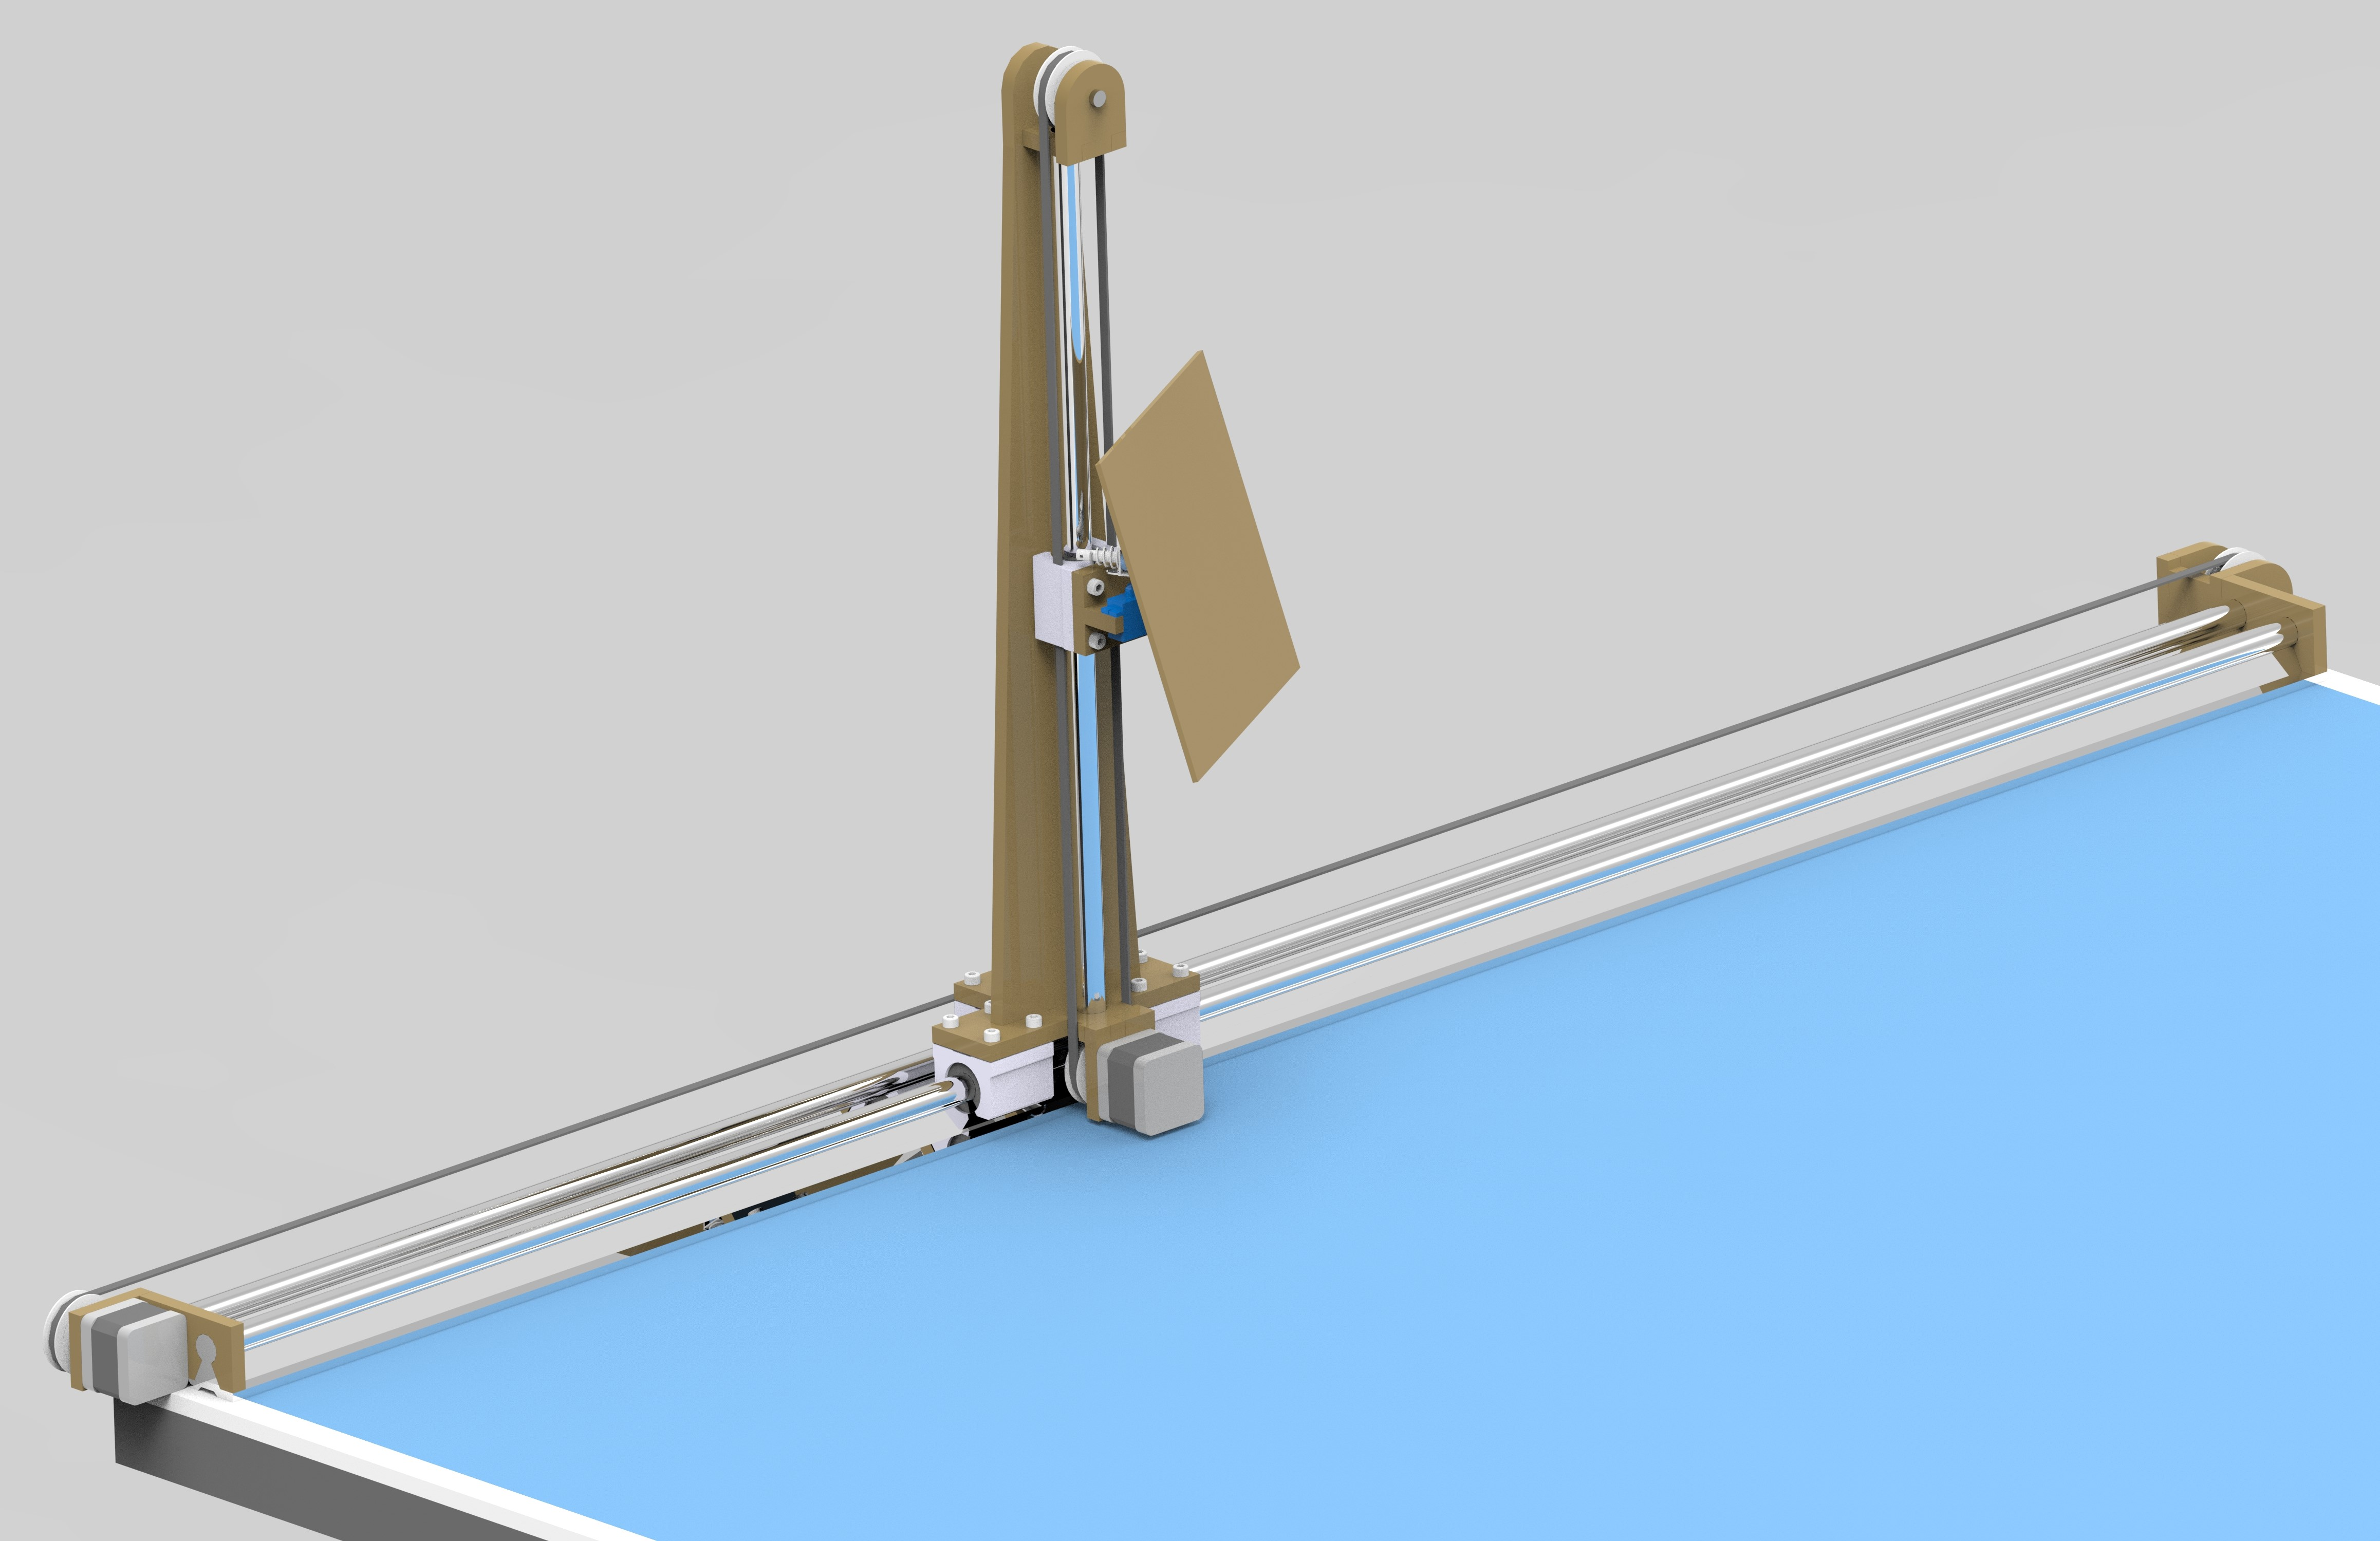
\includegraphics[height=5cm]{./images/frontrender.jpg}
	\caption{A render of the mechanical design from the front.}
\end{figure}
\begin{figure}[h] 
	\centering 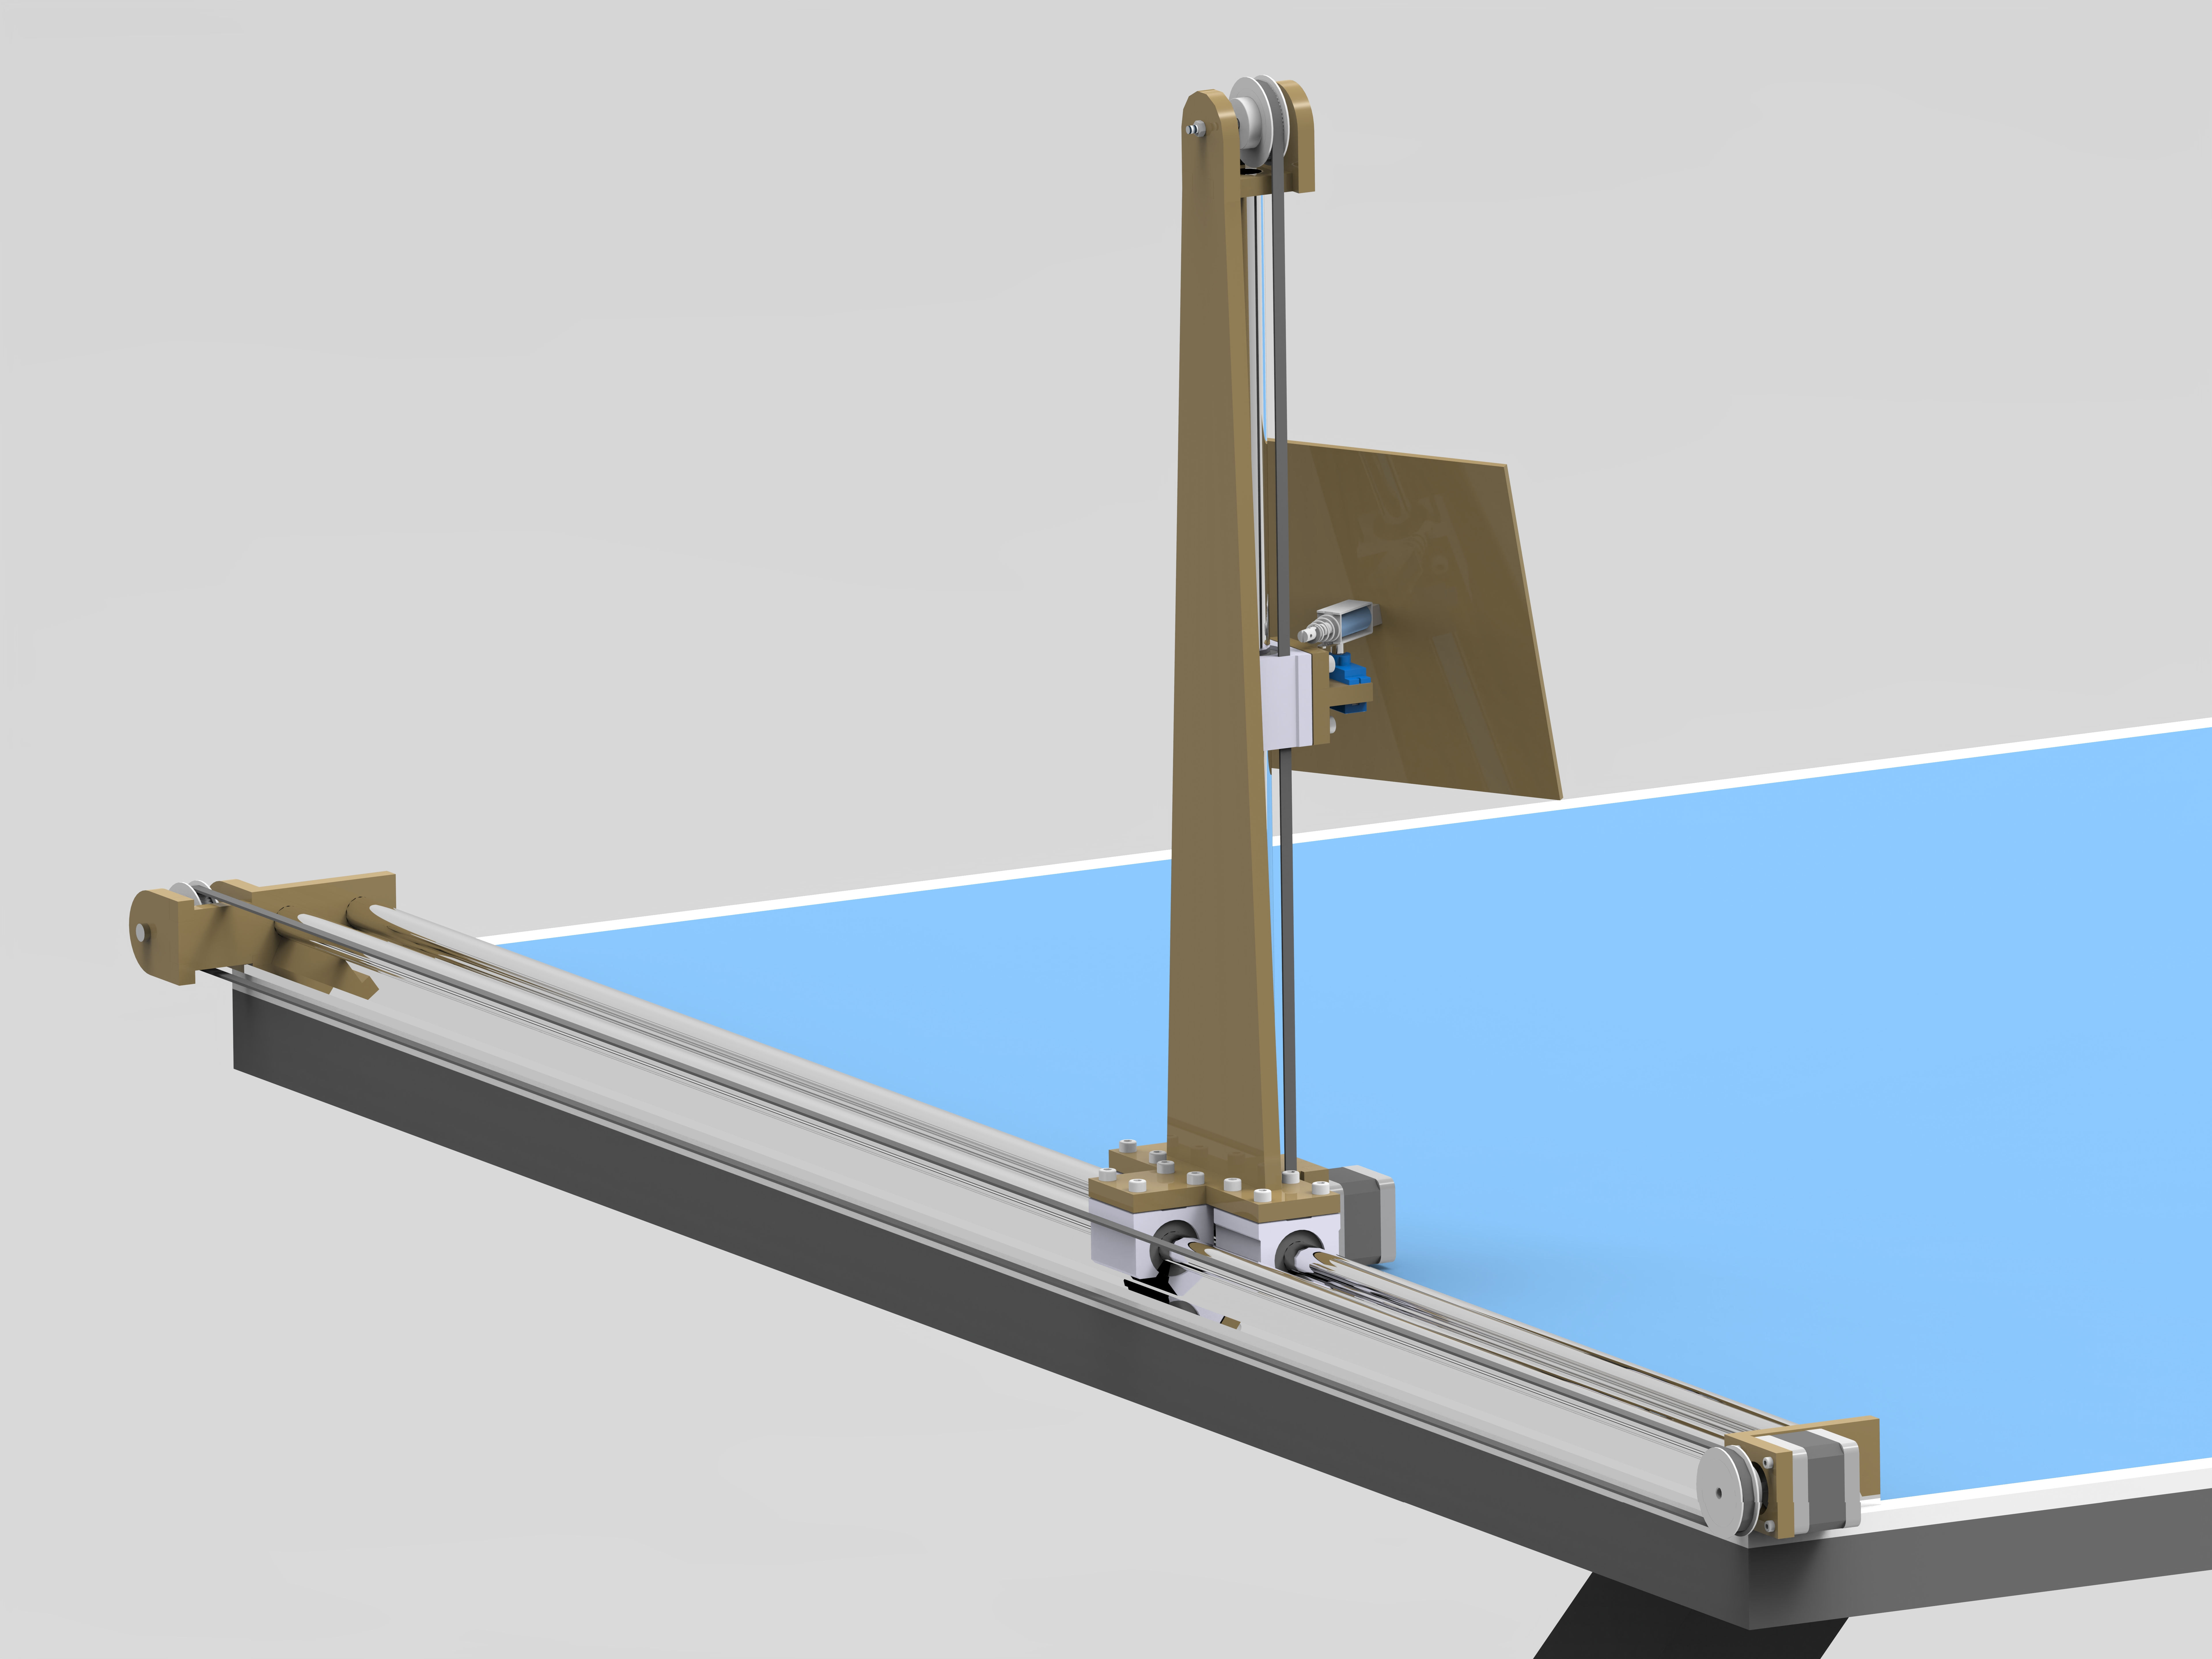
\includegraphics[height=5cm]{./images/backrender.jpg}
	\caption{A render of the mechanical design from the back.}
\end{figure}



\section{Block Diagram}
Below is a block diagram showing the general control flow of the entire system and all its components.

\begin{figure}[h]
	\centering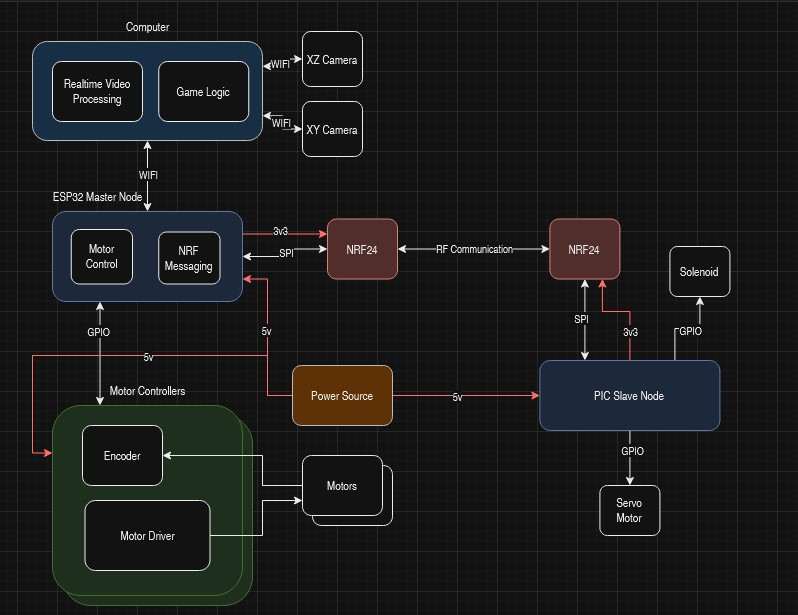
\includegraphics[height=6cm]{./images/blockdiagram}
	\caption{System Design Block Diagram}
\end{figure}

\section{Electronic Components and Controllers}
The system mainly relies on two mobile phones which are used for collecting the position information of the ping pong ball with three degrees of freedom. The mobile phones are configured with an app to act as IP cameras, which are then accessed over Wi-Fi on the control device, which is a laptop running our software.

The ESP32 microcontroller is connected to two stepper motor driver modules (DRV8825), which are in turn connected to two bipolar stepper motors which control the gantry. The ESP32 acts as a master to a PIC18F, through a connected radio frequency communication module (NRF24), which is used to transmit data to another NRF24 module, connected to the PIC18F slave microcontroller. This data consists of information on when to "fire" the racket to hit the ball, by activating the optocoupled 12V solenoid, and information on what angle the racket should be at, by controlling the 5V servo motor.

\section{Software Design}
The main software which controls the system is ran on a separate computer, due to the speed and computational constraints of small microcontrollers. The code connects to the IP camera phones, reads the streamed video data, and processes it using a computer vision algorithm and ball detection algorithms to determine the position of the ping pong ball in 3D space. The software sends a requested gantry position, a requested racket orientation, and when the racket should "fire" over Wi-Fi to the ESP32 microcontroller. Part of this data is then sent from over radio using the NRF24 from the ESP32 to the PIC18F.

The software additionally maintains the game state through a simplified rule-set, allowing the score and current ball position to be visualized in real time. The software determines the ball's position and additionally applies a predictive model to determine where the gantry should move to.


\section{Bill of Materials}

\textbf{!!! NEED TO BE UPDATED !!!}

\begin{center}
\begin{tabular}{|l|c|c|c|}
 \hline
Item & Amount & Unit Price (\texteuro) \\
 \hline\hline
 MDF (60x30) & 1 & 4 \\ 
 \hline
 5meter 6mm Timing Belt & 1 & 6.62\\
 \hline
 GT2 60-tooth gear & 4 & 3.19\\
 \hline
 0.5meter M16 Aluminium pipe & 2 & 5.9\\
 \hline
 1.5meter SBR16 Linear rail & 2 & 20.46\\
 \hline
 D5 M4 50mm Shoulder bolt & 2 & 2.94\\
 \hline
 Servo Motor & 1 & 3.5 \\
 \hline
 Solenoid & 1 & 6.9 \\ 
 \hline
 ESP32 & 1 & 6.9 \\
 \hline
 PIC18F & 1 & 2.4 \\
 \hline
 NRF24 & 2 & 6.68 \\
 \hline
 Stepper Motor & 3 & - \\
 \hline
 Stepper Driver DRV8825 & 3 & 13.5 \\
 \hline
 Optocoupler & 1 & - \\
 \hline
 Transistors & - & - \\
 \hline
 Resistors & - & - \\
 \hline
 Capacitors & - & - \\
 \hline
\end{tabular}
\end{center}